% Generated by Sphinx.
\def\sphinxdocclass{report}
\documentclass[letterpaper,10pt,english]{sphinxmanual}
\usepackage[utf8]{inputenc}
\DeclareUnicodeCharacter{00A0}{\nobreakspace}
\usepackage{cmap}
\usepackage[T1]{fontenc}
\usepackage{babel}
\usepackage{times}
\usepackage[Bjarne]{fncychap}
\usepackage{longtable}
\usepackage{sphinx}
\usepackage{multirow}

\addto\captionsenglish{\renewcommand{\figurename}{Fig. }}
\addto\captionsenglish{\renewcommand{\tablename}{Table }}
\floatname{literal-block}{Listing }



\title{K\_means Documentation}
\date{October 21, 2015}
\release{1.0}
\author{B. Pacreau, G. Soulié}
\newcommand{\sphinxlogo}{}
\renewcommand{\releasename}{Release}
\makeindex

\makeatletter
\def\PYG@reset{\let\PYG@it=\relax \let\PYG@bf=\relax%
    \let\PYG@ul=\relax \let\PYG@tc=\relax%
    \let\PYG@bc=\relax \let\PYG@ff=\relax}
\def\PYG@tok#1{\csname PYG@tok@#1\endcsname}
\def\PYG@toks#1+{\ifx\relax#1\empty\else%
    \PYG@tok{#1}\expandafter\PYG@toks\fi}
\def\PYG@do#1{\PYG@bc{\PYG@tc{\PYG@ul{%
    \PYG@it{\PYG@bf{\PYG@ff{#1}}}}}}}
\def\PYG#1#2{\PYG@reset\PYG@toks#1+\relax+\PYG@do{#2}}

\expandafter\def\csname PYG@tok@gd\endcsname{\def\PYG@tc##1{\textcolor[rgb]{0.63,0.00,0.00}{##1}}}
\expandafter\def\csname PYG@tok@gu\endcsname{\let\PYG@bf=\textbf\def\PYG@tc##1{\textcolor[rgb]{0.50,0.00,0.50}{##1}}}
\expandafter\def\csname PYG@tok@gt\endcsname{\def\PYG@tc##1{\textcolor[rgb]{0.00,0.27,0.87}{##1}}}
\expandafter\def\csname PYG@tok@gs\endcsname{\let\PYG@bf=\textbf}
\expandafter\def\csname PYG@tok@gr\endcsname{\def\PYG@tc##1{\textcolor[rgb]{1.00,0.00,0.00}{##1}}}
\expandafter\def\csname PYG@tok@cm\endcsname{\let\PYG@it=\textit\def\PYG@tc##1{\textcolor[rgb]{0.25,0.50,0.56}{##1}}}
\expandafter\def\csname PYG@tok@vg\endcsname{\def\PYG@tc##1{\textcolor[rgb]{0.73,0.38,0.84}{##1}}}
\expandafter\def\csname PYG@tok@m\endcsname{\def\PYG@tc##1{\textcolor[rgb]{0.13,0.50,0.31}{##1}}}
\expandafter\def\csname PYG@tok@mh\endcsname{\def\PYG@tc##1{\textcolor[rgb]{0.13,0.50,0.31}{##1}}}
\expandafter\def\csname PYG@tok@cs\endcsname{\def\PYG@tc##1{\textcolor[rgb]{0.25,0.50,0.56}{##1}}\def\PYG@bc##1{\setlength{\fboxsep}{0pt}\colorbox[rgb]{1.00,0.94,0.94}{\strut ##1}}}
\expandafter\def\csname PYG@tok@ge\endcsname{\let\PYG@it=\textit}
\expandafter\def\csname PYG@tok@vc\endcsname{\def\PYG@tc##1{\textcolor[rgb]{0.73,0.38,0.84}{##1}}}
\expandafter\def\csname PYG@tok@il\endcsname{\def\PYG@tc##1{\textcolor[rgb]{0.13,0.50,0.31}{##1}}}
\expandafter\def\csname PYG@tok@go\endcsname{\def\PYG@tc##1{\textcolor[rgb]{0.20,0.20,0.20}{##1}}}
\expandafter\def\csname PYG@tok@cp\endcsname{\def\PYG@tc##1{\textcolor[rgb]{0.00,0.44,0.13}{##1}}}
\expandafter\def\csname PYG@tok@gi\endcsname{\def\PYG@tc##1{\textcolor[rgb]{0.00,0.63,0.00}{##1}}}
\expandafter\def\csname PYG@tok@gh\endcsname{\let\PYG@bf=\textbf\def\PYG@tc##1{\textcolor[rgb]{0.00,0.00,0.50}{##1}}}
\expandafter\def\csname PYG@tok@ni\endcsname{\let\PYG@bf=\textbf\def\PYG@tc##1{\textcolor[rgb]{0.84,0.33,0.22}{##1}}}
\expandafter\def\csname PYG@tok@nl\endcsname{\let\PYG@bf=\textbf\def\PYG@tc##1{\textcolor[rgb]{0.00,0.13,0.44}{##1}}}
\expandafter\def\csname PYG@tok@nn\endcsname{\let\PYG@bf=\textbf\def\PYG@tc##1{\textcolor[rgb]{0.05,0.52,0.71}{##1}}}
\expandafter\def\csname PYG@tok@no\endcsname{\def\PYG@tc##1{\textcolor[rgb]{0.38,0.68,0.84}{##1}}}
\expandafter\def\csname PYG@tok@na\endcsname{\def\PYG@tc##1{\textcolor[rgb]{0.25,0.44,0.63}{##1}}}
\expandafter\def\csname PYG@tok@nb\endcsname{\def\PYG@tc##1{\textcolor[rgb]{0.00,0.44,0.13}{##1}}}
\expandafter\def\csname PYG@tok@nc\endcsname{\let\PYG@bf=\textbf\def\PYG@tc##1{\textcolor[rgb]{0.05,0.52,0.71}{##1}}}
\expandafter\def\csname PYG@tok@nd\endcsname{\let\PYG@bf=\textbf\def\PYG@tc##1{\textcolor[rgb]{0.33,0.33,0.33}{##1}}}
\expandafter\def\csname PYG@tok@ne\endcsname{\def\PYG@tc##1{\textcolor[rgb]{0.00,0.44,0.13}{##1}}}
\expandafter\def\csname PYG@tok@nf\endcsname{\def\PYG@tc##1{\textcolor[rgb]{0.02,0.16,0.49}{##1}}}
\expandafter\def\csname PYG@tok@si\endcsname{\let\PYG@it=\textit\def\PYG@tc##1{\textcolor[rgb]{0.44,0.63,0.82}{##1}}}
\expandafter\def\csname PYG@tok@s2\endcsname{\def\PYG@tc##1{\textcolor[rgb]{0.25,0.44,0.63}{##1}}}
\expandafter\def\csname PYG@tok@vi\endcsname{\def\PYG@tc##1{\textcolor[rgb]{0.73,0.38,0.84}{##1}}}
\expandafter\def\csname PYG@tok@nt\endcsname{\let\PYG@bf=\textbf\def\PYG@tc##1{\textcolor[rgb]{0.02,0.16,0.45}{##1}}}
\expandafter\def\csname PYG@tok@nv\endcsname{\def\PYG@tc##1{\textcolor[rgb]{0.73,0.38,0.84}{##1}}}
\expandafter\def\csname PYG@tok@s1\endcsname{\def\PYG@tc##1{\textcolor[rgb]{0.25,0.44,0.63}{##1}}}
\expandafter\def\csname PYG@tok@gp\endcsname{\let\PYG@bf=\textbf\def\PYG@tc##1{\textcolor[rgb]{0.78,0.36,0.04}{##1}}}
\expandafter\def\csname PYG@tok@sh\endcsname{\def\PYG@tc##1{\textcolor[rgb]{0.25,0.44,0.63}{##1}}}
\expandafter\def\csname PYG@tok@ow\endcsname{\let\PYG@bf=\textbf\def\PYG@tc##1{\textcolor[rgb]{0.00,0.44,0.13}{##1}}}
\expandafter\def\csname PYG@tok@sx\endcsname{\def\PYG@tc##1{\textcolor[rgb]{0.78,0.36,0.04}{##1}}}
\expandafter\def\csname PYG@tok@bp\endcsname{\def\PYG@tc##1{\textcolor[rgb]{0.00,0.44,0.13}{##1}}}
\expandafter\def\csname PYG@tok@c1\endcsname{\let\PYG@it=\textit\def\PYG@tc##1{\textcolor[rgb]{0.25,0.50,0.56}{##1}}}
\expandafter\def\csname PYG@tok@kc\endcsname{\let\PYG@bf=\textbf\def\PYG@tc##1{\textcolor[rgb]{0.00,0.44,0.13}{##1}}}
\expandafter\def\csname PYG@tok@c\endcsname{\let\PYG@it=\textit\def\PYG@tc##1{\textcolor[rgb]{0.25,0.50,0.56}{##1}}}
\expandafter\def\csname PYG@tok@mf\endcsname{\def\PYG@tc##1{\textcolor[rgb]{0.13,0.50,0.31}{##1}}}
\expandafter\def\csname PYG@tok@err\endcsname{\def\PYG@bc##1{\setlength{\fboxsep}{0pt}\fcolorbox[rgb]{1.00,0.00,0.00}{1,1,1}{\strut ##1}}}
\expandafter\def\csname PYG@tok@mb\endcsname{\def\PYG@tc##1{\textcolor[rgb]{0.13,0.50,0.31}{##1}}}
\expandafter\def\csname PYG@tok@ss\endcsname{\def\PYG@tc##1{\textcolor[rgb]{0.32,0.47,0.09}{##1}}}
\expandafter\def\csname PYG@tok@sr\endcsname{\def\PYG@tc##1{\textcolor[rgb]{0.14,0.33,0.53}{##1}}}
\expandafter\def\csname PYG@tok@mo\endcsname{\def\PYG@tc##1{\textcolor[rgb]{0.13,0.50,0.31}{##1}}}
\expandafter\def\csname PYG@tok@kd\endcsname{\let\PYG@bf=\textbf\def\PYG@tc##1{\textcolor[rgb]{0.00,0.44,0.13}{##1}}}
\expandafter\def\csname PYG@tok@mi\endcsname{\def\PYG@tc##1{\textcolor[rgb]{0.13,0.50,0.31}{##1}}}
\expandafter\def\csname PYG@tok@kn\endcsname{\let\PYG@bf=\textbf\def\PYG@tc##1{\textcolor[rgb]{0.00,0.44,0.13}{##1}}}
\expandafter\def\csname PYG@tok@o\endcsname{\def\PYG@tc##1{\textcolor[rgb]{0.40,0.40,0.40}{##1}}}
\expandafter\def\csname PYG@tok@kr\endcsname{\let\PYG@bf=\textbf\def\PYG@tc##1{\textcolor[rgb]{0.00,0.44,0.13}{##1}}}
\expandafter\def\csname PYG@tok@s\endcsname{\def\PYG@tc##1{\textcolor[rgb]{0.25,0.44,0.63}{##1}}}
\expandafter\def\csname PYG@tok@kp\endcsname{\def\PYG@tc##1{\textcolor[rgb]{0.00,0.44,0.13}{##1}}}
\expandafter\def\csname PYG@tok@w\endcsname{\def\PYG@tc##1{\textcolor[rgb]{0.73,0.73,0.73}{##1}}}
\expandafter\def\csname PYG@tok@kt\endcsname{\def\PYG@tc##1{\textcolor[rgb]{0.56,0.13,0.00}{##1}}}
\expandafter\def\csname PYG@tok@sc\endcsname{\def\PYG@tc##1{\textcolor[rgb]{0.25,0.44,0.63}{##1}}}
\expandafter\def\csname PYG@tok@sb\endcsname{\def\PYG@tc##1{\textcolor[rgb]{0.25,0.44,0.63}{##1}}}
\expandafter\def\csname PYG@tok@k\endcsname{\let\PYG@bf=\textbf\def\PYG@tc##1{\textcolor[rgb]{0.00,0.44,0.13}{##1}}}
\expandafter\def\csname PYG@tok@se\endcsname{\let\PYG@bf=\textbf\def\PYG@tc##1{\textcolor[rgb]{0.25,0.44,0.63}{##1}}}
\expandafter\def\csname PYG@tok@sd\endcsname{\let\PYG@it=\textit\def\PYG@tc##1{\textcolor[rgb]{0.25,0.44,0.63}{##1}}}

\def\PYGZbs{\char`\\}
\def\PYGZus{\char`\_}
\def\PYGZob{\char`\{}
\def\PYGZcb{\char`\}}
\def\PYGZca{\char`\^}
\def\PYGZam{\char`\&}
\def\PYGZlt{\char`\<}
\def\PYGZgt{\char`\>}
\def\PYGZsh{\char`\#}
\def\PYGZpc{\char`\%}
\def\PYGZdl{\char`\$}
\def\PYGZhy{\char`\-}
\def\PYGZsq{\char`\'}
\def\PYGZdq{\char`\"}
\def\PYGZti{\char`\~}
% for compatibility with earlier versions
\def\PYGZat{@}
\def\PYGZlb{[}
\def\PYGZrb{]}
\makeatother

\renewcommand\PYGZsq{\textquotesingle}

\begin{document}

\maketitle
\tableofcontents
\phantomsection\label{index::doc}


L'ensemble des sources de ce projet est disponible sur \href{http://github.com/pikkendorff/kmeans}{github} :

Sous linux, vous pouvez facilement l'importer en tapant :
\begin{quote}

\begin{Verbatim}[commandchars=\\\{\}]
\PYG{n}{mkdir} \PYG{n}{kmeans}\PYG{o}{/}
\PYG{n}{cd} \PYG{n}{kmeans}
\PYG{n}{git} \PYG{n}{init}
\PYG{n}{git} \PYG{n}{remote} \PYG{n}{http}\PYG{p}{:}\PYG{o}{/}\PYG{o}{/}\PYG{n}{github}\PYG{o}{.}\PYG{n}{com}\PYG{o}{/}\PYG{n}{pikkendorff}\PYG{o}{/}\PYG{n}{kmeans} \PYG{n}{master}
\end{Verbatim}
\end{quote}

L'architecture générale du projet est la suivante :
\begin{quote}

\begin{Verbatim}[commandchars=\\\{\}]
./kmeans/
      \textbar{}\PYGZhy{}\PYGZhy{}doc/
      \textbar{}\PYGZhy{}\PYGZhy{}input/
      \textbar{}    \textbar{}\PYGZhy{}\PYGZhy{}input.csv
      \textbar{}    \textbar{}\PYGZhy{}\PYGZhy{}bretagne.jpg
      \textbar{}    \textbar{}\PYGZhy{}\PYGZhy{}.iris.csv
      \textbar{}\PYGZhy{}\PYGZhy{}output/
      \textbar{}    \textbar{}\PYGZhy{}\PYGZhy{}affectation.csv
      \textbar{}    \textbar{}\PYGZhy{}\PYGZhy{}centroids.csv
      \textbar{}\PYGZhy{}\PYGZhy{}kmeans.py
      \textbar{}\PYGZhy{}\PYGZhy{}es.py
      \textbar{}\PYGZhy{}\PYGZhy{}genData.py
      \textbar{}\PYGZhy{}\PYGZhy{}Observation.py
\end{Verbatim}
\end{quote}

Lorsqu'on lance kmeans, les données présentes dans le fichier \emph{./input/input.csv} sont étudiées, et le résultat est écrit dans deux fichiers, \emph{./output/affectation.csv} et \emph{./output/centroids.csv}

Les fichiers \emph{\{genAleatoire}, \emph{genIris} et \emph{genPicture\}.py} vous permettent de générer un fichier input.csv corrsespondant respectivement aux sections {\hyperref[nD:random]{\emph{\DUspan{}{Données aléatoires}}}}, {\hyperref[iris:iris]{\emph{\DUspan{}{Données Iris}}}} et {\hyperref[sky:sky]{\emph{\DUspan{}{La Bretagne vue du ciel}}}}. Bien évidemment, vous pouvez utiliser l'algorithme avec un autre jeu de données de votre choix, pourvu que le fichier \emph{input.csv} respecte le bon format (cf {\hyperref[data:format]{\emph{\DUspan{}{Format des données}}}}).


\chapter{Table des matières}
\label{index:table-des-matieres}\label{index:documentation-du-projet-k-means}

\section{Introduction}
\label{introduction:introduction}\label{introduction::doc}
Selon Wikipédia, ``Le partitionnement en k-moyennes (ou k-means en anglais) est une méthode de partitionnement de données et un problème d'optimisation combinatoire''. Ceci étant dit, prenons le temps de présenter de manière plus général le contexte dans lequel cet algorithme est généralement utilisé : l'apprentissage automatique


\subsection{Apprentissage Automatique (\emph{Machine learning})}
\label{introduction:apprentissage-automatique-machine-learning}
L'apprentissage automatique, plus connu sous le nom de \emph{machine learning} en Anglais, est un sous-domaine de l'intelligence artificielle qui vise à effectuer des actions pour lesquelles ils n'ont pas été explicitement programés. Concrétement, on distingue l'apprentissage supervisé de l'apprentissage non supervisé.
\begin{itemize}
\item {} 
Apprentissage supervisé (\emph{supervised learning}) : Consiste à attribuer une étiquette (\emph{label}) à des données.

\item {} 
Apprentissage non supervisé (\emph{unsupervised learning}) : Consiste à séparer un ensemble de données en plusieurs catégories

\end{itemize}


\subsection{Apprentissage supervisé}
\label{introduction:apprentissage-supervise}
C'est le cas par exemple des célébres de classification d'image du type reconnaissance de chiffres manuscrit (\href{http://yann.lecun.com/exdb/mnist/index.html}{MNIST}), d'images(\href{http://www.image-net.org/}{ImageNet}). C'est également le cas si l'on veut determiner le prix d'un appartement en fonction de ses caractéristiques, ou encore la gravité d'une tumeur.

Le principe de fonctionnement est simple : on utilise un grand ensemble de données déjà étiquetée (appelé ensemble d'entrainement) pour construire un modèle, qui nous servira ensuite a estimer l'étiquette d'une donnée non étiquetée. Un jeu de données étiquetées (appelé ensemble de test), non utilisées pour l'entrainement du réseau, nous sert à vérifier la validité du modèle :

{\hfill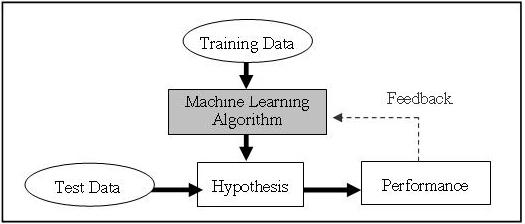
\includegraphics{AA_diagramm.jpg}\hfill}

Parmi les grands algorithmes d'apprentissage supervisé, on compte les réseaux de neurones.


\subsection{Apprentissage non supervisé}
\label{introduction:apprentissage-non-supervise}
L'exemple classique pour évoquer l'apprentissage non supervisé concerne la segmentation du marché d'une entreprise. Une entreprise possède un certains nombre de clients et aimerait les dissocier en plusieurs catégories, mais ne connait pas forcément le nombre, la taille ou le type de catégorie à l'avance. Il s'agit de trouver un `juste milieu' entre prendre une catégorie par individu, et une pour tous.

Un autre exemple que nous proposons, est celui d'une compagnie des Telecom qui voudrait installer un réseau d'antennes en Bretagne. Ne disposant que d'un nombre limité d'antennes, la compagnie souhaite maximiser l'emplacement de celles-ci. Une solution pour elle est de faire appel à un algorithme d'apprentissage non supervisé pour séparer la population en différentes catégories, et ensuite disposer une antenne pour chaque catégorie.
Il s'agit donc de détecter une structure cachée dans l'ensemble de données.

L'un des algorithmes les plus célèbres pour faire de l'apprentissage non supervisé est précisemment l'algorithme des k-moyennes, plus connus sous son nom anglais \emph{k-means}.

En particulier, nous allons étudier dans ce projet le deuxième exemple proposé : utiliser k-means pour positionner des antennes téléphoniques en Bretagne.


\section{Etude théorique de k-means}
\label{kmeans:imagenet}\label{kmeans:etude-theorique-de-k-means}\label{kmeans::doc}

\section{Implémentation de k-means}
\label{impl:module-kmeans}\label{impl::doc}\label{impl:implementation-de-k-means}\index{kmeans (module)}
Pour implémenter l'algorithme kmeans, nous avons utilisé deux fichiers :
kmeans.py et Observation.py

Le fichier kmeans contient la focntion compute\_kmeans


\subsection{La fonction compute\_kmeans}
\label{impl:la-fonction-compute-kmeans}\index{compute\_kmeans() (in module kmeans)}

\begin{fulllineitems}
\phantomsection\label{impl:kmeans.compute_kmeans}\pysiglinewithargsret{\code{kmeans.}\bfcode{compute\_kmeans}}{\emph{k}, \emph{display=False}, \emph{max\_iteration=99999}}{}~\begin{description}
\item[{Compute and display the k-means algorithm on the input file }] \leavevmode
(\emph{./input/input.csv})

\end{description}
\begin{quote}\begin{description}
\item[{Parameters}] \leavevmode\begin{itemize}
\item {} 
\textbf{\texttt{k}} (\emph{int}) -- the k of k-means : number of centroids

\item {} 
\textbf{\texttt{max\_iteration}} (\emph{int}) -- the number maximum of iteration we allow

\item {} 
\textbf{\texttt{display}} (\emph{boolean}) -- if True, the first and the second coordinate of the 
populations are displayed setep by step

\end{itemize}

\end{description}\end{quote}

\end{fulllineitems}


compute\_kmeans fait appel au fichier es.py qui regroupe l'ensemble des
opérations d'écriture, de lecture et d'affichages des {\hyperref[data:data]{\emph{\DUspan{}{données}}}}

\begin{Verbatim}[commandchars=\\\{\}]
\PYG{n}{population} \PYG{o}{=} \PYG{n}{es}\PYG{o}{.}\PYG{n}{read\PYGZus{}kmeans\PYGZus{}input}\PYG{p}{(}\PYG{p}{)}
\PYG{n}{dimension} \PYG{o}{=} \PYG{n+nb}{len}\PYG{p}{(}\PYG{n}{population}\PYG{p}{[}\PYG{l+m+mi}{0}\PYG{p}{]}\PYG{o}{.}\PYG{n}{values}\PYG{p}{)}
\end{Verbatim}


\subsubsection{Phase 1 - Initialisation}
\label{impl:phase-1-initialisation}\begin{quote}

\begin{Verbatim}[commandchars=\\\{\}]
\PYG{c}{\PYGZsh{}centroids initialisation:}
\PYG{n}{centroids}\PYG{o}{=}\PYG{p}{[}\PYG{p}{]}
\PYG{n}{isSelected}\PYG{o}{=}\PYG{p}{[}\PYG{p}{]}
\PYG{k}{for} \PYG{n}{i} \PYG{o+ow}{in} \PYG{n+nb}{range}\PYG{p}{(}\PYG{n+nb}{len}\PYG{p}{(}\PYG{n}{population}\PYG{p}{)}\PYG{p}{)}\PYG{p}{:}
        \PYG{n}{isSelected}\PYG{o}{.}\PYG{n}{append}\PYG{p}{(}\PYG{l+m+mi}{0}\PYG{p}{)}
\PYG{k}{for} \PYG{n}{i} \PYG{o+ow}{in} \PYG{n+nb}{range}\PYG{p}{(}\PYG{n}{k}\PYG{p}{)}\PYG{p}{:}
        \PYG{k}{while} \PYG{n+nb+bp}{True}\PYG{p}{:}

                \PYG{c}{\PYGZsh{}centroids are ranomly choose in the population}
                \PYG{n}{index} \PYG{o}{=} \PYG{n+nb}{int}\PYG{p}{(}\PYG{n}{floor}\PYG{p}{(}\PYG{n}{random}\PYG{o}{.}\PYG{n}{random}\PYG{p}{(}\PYG{p}{)}\PYG{o}{*}\PYG{n+nb}{len}\PYG{p}{(}\PYG{n}{population}\PYG{p}{)}\PYG{p}{)}\PYG{p}{)}

                \PYG{c}{\PYGZsh{}We checked that we don\PYGZsq{}t take the same centroid twice}
                \PYG{k}{if} \PYG{n}{isSelected}\PYG{p}{[}\PYG{n}{index}\PYG{p}{]}\PYG{o}{==}\PYG{l+m+mi}{0}\PYG{p}{:}
                        \PYG{n}{centroids}\PYG{o}{.}\PYG{n}{append}\PYG{p}{(}\PYG{n}{population}\PYG{p}{[}\PYG{n}{index}\PYG{p}{]}\PYG{o}{.}\PYG{n}{copy}\PYG{p}{(}\PYG{p}{)}\PYG{p}{)}
                        \PYG{n}{isSelected}\PYG{p}{[}\PYG{n}{index}\PYG{p}{]}\PYG{o}{=}\PYG{l+m+mi}{1}
                        \PYG{k}{break}

\PYG{c}{\PYGZsh{}affectation initialisation:}
\PYG{n}{affectation}\PYG{o}{=}\PYG{p}{[}\PYG{p}{]}
\PYG{k}{for} \PYG{n}{i} \PYG{o+ow}{in} \PYG{n+nb}{range}\PYG{p}{(}\PYG{n+nb}{len}\PYG{p}{(}\PYG{n}{population}\PYG{p}{)}\PYG{p}{)}\PYG{p}{:}
        \PYG{n}{affectation}\PYG{o}{.}\PYG{n}{append}\PYG{p}{(}\PYG{l+m+mi}{0}\PYG{p}{)}
\PYG{k}{if} \PYG{n}{display}\PYG{p}{:}
        \PYG{n}{es}\PYG{o}{.}\PYG{n}{display}\PYG{p}{(}\PYG{n}{population}\PYG{p}{,}\PYG{n+nb+bp}{None}\PYG{p}{,}\PYG{l+s}{\PYGZdq{}}\PYG{l+s}{Population : }\PYG{l+s}{\PYGZdq{}}\PYG{p}{)}

\PYG{c}{\PYGZsh{}Loop stop condition initialisation:}
\PYG{n}{stop}\PYG{o}{=}\PYG{n+nb+bp}{False}


\PYG{n}{iteration} \PYG{o}{=} \PYG{l+m+mi}{0}
\PYG{k}{while} \PYG{o+ow}{not} \PYG{n}{stop} \PYG{o+ow}{and} \PYG{n}{iteration} \PYG{o}{\PYGZlt{}} \PYG{n}{max\PYGZus{}iteration}\PYG{p}{:}
        \PYG{n}{iteration}\PYG{o}{+}\PYG{o}{=}\PYG{l+m+mi}{1}
\end{Verbatim}
\end{quote}


\subsubsection{Phase 2 - Affectation}
\label{impl:phase-2-affectation}\begin{quote}

\begin{Verbatim}[commandchars=\\\{\}]
\PYG{c}{\PYGZsh{}if display, we print the population and the centroids}
\PYG{k}{if} \PYG{n}{display}\PYG{p}{:}
        \PYG{n}{es}\PYG{o}{.}\PYG{n}{display}\PYG{p}{(}\PYG{n}{population}\PYG{p}{,}\PYG{n}{centroids}\PYG{p}{,}\PYG{l+s}{\PYGZdq{}}\PYG{l+s}{computing k\PYGZhy{}means : }\PYG{l+s+se}{\PYGZbs{}}
\PYG{l+s}{                iteration }\PYG{l+s}{\PYGZdq{}}\PYG{o}{+}\PYG{n+nb}{str}\PYG{p}{(}\PYG{n}{iteration}\PYG{p}{)}\PYG{p}{)}

\PYG{c}{\PYGZsh{}Compute the distance between each observation and each centroid}
\PYG{n}{distance}\PYG{o}{=}\PYG{p}{[}\PYG{p}{[}\PYG{p}{]}\PYG{p}{]}
\PYG{k}{for} \PYG{n}{i} \PYG{o+ow}{in} \PYG{n+nb}{range}\PYG{p}{(}\PYG{n+nb}{len}\PYG{p}{(}\PYG{n}{population}\PYG{p}{)}\PYG{p}{)}\PYG{p}{:}
        \PYG{n}{distance}\PYG{o}{.}\PYG{n}{append}\PYG{p}{(}\PYG{p}{[}\PYG{p}{]}\PYG{p}{)}
        \PYG{k}{for} \PYG{n}{j} \PYG{o+ow}{in} \PYG{n+nb}{range}\PYG{p}{(}\PYG{n}{k}\PYG{p}{)}\PYG{p}{:}
                \PYG{n}{distance}\PYG{p}{[}\PYG{n}{i}\PYG{p}{]}\PYG{o}{.}\PYG{n}{append}\PYG{p}{(}\PYG{n}{population}\PYG{p}{[}\PYG{n}{i}\PYG{p}{]}\PYG{o}{.}\PYG{n}{dist}\PYG{p}{(}\PYG{n}{centroids}\PYG{p}{[}\PYG{n}{j}\PYG{p}{]}\PYG{p}{)}\PYG{p}{)}

\PYG{c}{\PYGZsh{}The loop stop condition is fixed to True}
\PYG{n}{stop} \PYG{o}{=} \PYG{n+nb+bp}{True}

\PYG{c}{\PYGZsh{}Affect the nearest centroid to each observation.}
\PYG{k}{for} \PYG{n}{i} \PYG{o+ow}{in} \PYG{n+nb}{range}\PYG{p}{(}\PYG{n+nb}{len}\PYG{p}{(}\PYG{n}{population}\PYG{p}{)}\PYG{p}{)}\PYG{p}{:}
        \PYG{n}{index\PYGZus{}du\PYGZus{}minimum} \PYG{o}{=} \PYG{n}{distance}\PYG{p}{[}\PYG{n}{i}\PYG{p}{]}\PYG{o}{.}\PYG{n}{index}\PYG{p}{(}\PYG{n+nb}{min}\PYG{p}{(}\PYG{n}{distance}\PYG{p}{[}\PYG{n}{i}\PYG{p}{]}\PYG{p}{)}\PYG{p}{)}
        \PYG{k}{if} \PYG{o+ow}{not} \PYG{n}{affectation}\PYG{p}{[}\PYG{n}{i}\PYG{p}{]}\PYG{o}{==}\PYG{n}{index\PYGZus{}du\PYGZus{}minimum}\PYG{p}{:}
                \PYG{n}{affectation}\PYG{p}{[}\PYG{n}{i}\PYG{p}{]}\PYG{o}{=}\PYG{n}{index\PYGZus{}du\PYGZus{}minimum}

\PYG{c}{\PYGZsh{}If there is any changement, the loop stop condition became false}
                \PYG{n}{stop} \PYG{o}{=} \PYG{n+nb+bp}{False}
\end{Verbatim}
\end{quote}


\subsubsection{Phase 3 - Calculation}
\label{impl:phase-3-calculation}\begin{quote}

\begin{Verbatim}[commandchars=\\\{\}]
\PYG{c}{\PYGZsh{}Compute the new centroids}
\PYG{k}{for} \PYG{n}{j} \PYG{o+ow}{in} \PYG{n+nb}{range}\PYG{p}{(}\PYG{n}{k}\PYG{p}{)}\PYG{p}{:}
        \PYG{n}{centroid} \PYG{o}{=} \PYG{n}{Observation}\PYG{p}{(}\PYG{n}{dimension}\PYG{p}{,}\PYG{n+nb}{type}\PYG{o}{=}\PYG{l+s}{\PYGZdq{}}\PYG{l+s}{centroid}\PYG{l+s}{\PYGZdq{}}\PYG{p}{)}
        \PYG{k}{for} \PYG{n}{i} \PYG{o+ow}{in} \PYG{n+nb}{range}\PYG{p}{(}\PYG{n+nb}{len}\PYG{p}{(}\PYG{n}{population}\PYG{p}{)}\PYG{p}{)}\PYG{p}{:}
                \PYG{k}{if} \PYG{n}{affectation}\PYG{p}{[}\PYG{n}{i}\PYG{p}{]}\PYG{o}{==}\PYG{n}{j}\PYG{p}{:}
                        \PYG{n}{centroid}\PYG{o}{.}\PYG{n}{add}\PYG{p}{(}\PYG{n}{population}\PYG{p}{[}\PYG{n}{i}\PYG{p}{]}\PYG{p}{)}
        \PYG{n}{centroids}\PYG{p}{[}\PYG{n}{j}\PYG{p}{]}\PYG{o}{=}\PYG{n}{centroid}
\end{Verbatim}
\end{quote}

\begin{Verbatim}[commandchars=\\\{\}]
\PYG{c}{\PYGZsh{}write the output files}
\PYG{n}{es}\PYG{o}{.}\PYG{n}{write\PYGZus{}kmeans\PYGZus{}output}\PYG{p}{(}\PYG{n}{population}\PYG{p}{,}\PYG{n}{centroids}\PYG{p}{,}\PYG{n}{affectation}\PYG{p}{)}

\PYG{c}{\PYGZsh{}if display, we print the population and the centroids}
\PYG{k}{if} \PYG{n}{display}\PYG{p}{:}
        \PYG{n}{es}\PYG{o}{.}\PYG{n}{display}\PYG{p}{(}\PYG{n}{population}\PYG{p}{,}\PYG{n}{centroids}\PYG{p}{,}\PYG{l+s}{\PYGZdq{}}\PYG{l+s}{K\PYGZhy{}means computed}\PYG{l+s}{\PYGZdq{}}\PYG{p}{)}
\end{Verbatim}


\subsection{La classe Observation}
\label{impl:la-classe-observation}\index{Observation (class in kmeans)}

\begin{fulllineitems}
\phantomsection\label{impl:kmeans.Observation}\pysiglinewithargsret{\strong{class }\code{kmeans.}\bfcode{Observation}}{\emph{dimension}}{}
Représente une observation
\index{\_\_init\_\_() (kmeans.Observation method)}

\begin{fulllineitems}
\phantomsection\label{impl:kmeans.Observation.__init__}\pysiglinewithargsret{\bfcode{\_\_init\_\_}}{\emph{dimension}}{}
Create a new observation.
\begin{quote}\begin{description}
\item[{Parameters}] \leavevmode
\textbf{\texttt{dimension}} (\emph{int}) -- dimension of the observation

\end{description}\end{quote}

\end{fulllineitems}

\index{add() (kmeans.Observation method)}

\begin{fulllineitems}
\phantomsection\label{impl:kmeans.Observation.add}\pysiglinewithargsret{\bfcode{add}}{\emph{observation}}{}
Add another observation values to self.values, with ponderation by self.weight.
Typically use wen this instanciation of Observation is a centroid.
This function permits to compute easily a barycentre of several observations
\begin{quote}\begin{description}
\item[{Parameters}] \leavevmode
\textbf{\texttt{observation}} ({\hyperref[impl:kmeans.Observation]{\emph{\emph{Observation}}}}) -- the observation to add to the barycentre

\end{description}\end{quote}

\end{fulllineitems}

\index{copy() (kmeans.Observation method)}

\begin{fulllineitems}
\phantomsection\label{impl:kmeans.Observation.copy}\pysiglinewithargsret{\bfcode{copy}}{}{}
Return another obseration with the same values
\begin{quote}\begin{description}
\item[{Return type}] \leavevmode
{\hyperref[impl:kmeans.Observation]{\emph{Observation}}}

\end{description}\end{quote}

\end{fulllineitems}

\index{dist() (kmeans.Observation method)}

\begin{fulllineitems}
\phantomsection\label{impl:kmeans.Observation.dist}\pysiglinewithargsret{\bfcode{dist}}{\emph{observation}}{}
compute and return the euclidian distance between self                  and another observation
\begin{quote}\begin{description}
\item[{Parameters}] \leavevmode
\textbf{\texttt{observation}} ({\hyperref[impl:kmeans.Observation]{\emph{\emph{Observation}}}}) -- the observation to compute the distance with

\item[{Return type}] \leavevmode
float

\end{description}\end{quote}

\end{fulllineitems}

\index{set\_values() (kmeans.Observation method)}

\begin{fulllineitems}
\phantomsection\label{impl:kmeans.Observation.set_values}\pysiglinewithargsret{\bfcode{set\_values}}{\emph{values}}{}
set the values of the observation
\begin{quote}\begin{description}
\item[{Parameters}] \leavevmode
\textbf{\texttt{values}} (\emph{float{[}{]}}) -- valeurs de l'observation

\item[{Return type}] \leavevmode
void

\end{description}\end{quote}

\end{fulllineitems}


\end{fulllineitems}



\section{Traitement des données}
\label{data:data}\label{data::doc}\label{data:traitement-des-donnees}

\subsection{Lire, écrire et afficher des données}
\label{data:lire-ecrire-et-afficher-des-donnees}
Le fichier \emph{es.py} regroupe l'ensemble des méthodes nécessaires à la lecture, à l'écriture et à l'affichage
des données.
\phantomsection\label{data:module-es}\index{es (module)}\index{display() (in module es)}

\begin{fulllineitems}
\phantomsection\label{data:es.display}\pysiglinewithargsret{\code{es.}\bfcode{display}}{\emph{population}, \emph{centroids}, \emph{title}, \emph{keep}}{}
This fonction is used to display the population and the centroids on a graph
\begin{quote}\begin{description}
\item[{Parameters}] \leavevmode\begin{itemize}
\item {} 
\textbf{\texttt{population}} (\emph{Observation{[}{]}}) -- set of observations

\item {} 
\textbf{\texttt{centroids}} (\emph{Observation{[}{]}}) -- set of centroids

\item {} 
\textbf{\texttt{titre}} (\emph{String}) -- name of the graphic

\end{itemize}

\end{description}\end{quote}

:arg    keep : if true, the figure stay open until the user close it
:type   keep : boolean
:rtype: void

\end{fulllineitems}

\index{read\_data() (in module es)}

\begin{fulllineitems}
\phantomsection\label{data:es.read_data}\pysiglinewithargsret{\code{es.}\bfcode{read\_data}}{\emph{filename}, \emph{skip\_first\_line=False}, \emph{ignore\_first\_column=False}}{}
Loads data from a csv file and returns the corresponding list.
All data are expected to be floats, except in the first column.
\begin{quote}\begin{description}
\item[{Parameters}] \leavevmode\begin{itemize}
\item {} 
\textbf{\texttt{filename}} (\emph{String}) -- csv file name.

\item {} 
\textbf{\texttt{skip\_first\_line}} (\emph{boolean}) -- if True, the first line is not read.
Default value: False.

\item {} 
\textbf{\texttt{ignore\_first\_column}} (\emph{boolean}) -- if True, the first column is ignored.
Default value: False.

\end{itemize}

\item[{Returns}] \leavevmode
a list of lists, each list being a row in the data file.
Rows are returned in the same order as in the file.
They contains floats, except for the 1st element which is a string
when the first column is not ignored.

\item[{Return type}] \leavevmode
float{[}{]}{[}{]}

\end{description}\end{quote}

\end{fulllineitems}

\index{read\_kmeans\_input() (in module es)}

\begin{fulllineitems}
\phantomsection\label{data:es.read_kmeans_input}\pysiglinewithargsret{\code{es.}\bfcode{read\_kmeans\_input}}{}{}
This fonction reads the file ``input.csv'' within the input folder
\begin{quote}\begin{description}
\item[{Returns}] \leavevmode
population based on the input file

\item[{Return type}] \leavevmode
Observation{[}{]}

\end{description}\end{quote}

\end{fulllineitems}

\index{write\_data() (in module es)}

\begin{fulllineitems}
\phantomsection\label{data:es.write_data}\pysiglinewithargsret{\code{es.}\bfcode{write\_data}}{\emph{data}, \emph{filename}}{}
Writes data in a csv file.
\begin{quote}\begin{description}
\item[{Parameters}] \leavevmode\begin{itemize}
\item {} 
\textbf{\texttt{data}} (\emph{float{[}{]}{[}{]}}) -- a list of lists to write

\item {} 
\textbf{\texttt{filename}} (\emph{String}) -- the path of the file in which data is written.
The file is created if necessary; if it exists, it is overwritten.

\end{itemize}

\end{description}\end{quote}

\end{fulllineitems}

\index{write\_kmeans\_input() (in module es)}

\begin{fulllineitems}
\phantomsection\label{data:es.write_kmeans_input}\pysiglinewithargsret{\code{es.}\bfcode{write\_kmeans\_input}}{\emph{population}, \emph{dimension}}{}
This function write the file \emph{input.csv} in the input folder
\begin{quote}\begin{description}
\item[{Parameters}] \leavevmode
\textbf{\texttt{population}} (\emph{float{[}{]}{[}{]}}) -- the set of observation we want to compute

\end{description}\end{quote}

\end{fulllineitems}

\index{write\_kmeans\_output() (in module es)}

\begin{fulllineitems}
\phantomsection\label{data:es.write_kmeans_output}\pysiglinewithargsret{\code{es.}\bfcode{write\_kmeans\_output}}{\emph{population}, \emph{centroids}, \emph{affectation}}{}
This fonction writes the files \emph{affectation.csv} and \emph{centroids.csv} in the output folder.
\begin{quote}\begin{description}
\item[{Parameters}] \leavevmode\begin{itemize}
\item {} 
\textbf{\texttt{population}} (\emph{Observation{[}{]}}) -- set of observations

\item {} 
\textbf{\texttt{centroids}} (\emph{Observation{[}{]}}) -- set of centroids

\item {} 
\textbf{\texttt{affectation}} (\emph{int{[}{]}}) -- list of the observation's centroid label

\end{itemize}

\item[{Return type}] \leavevmode
void

\end{description}\end{quote}

\end{fulllineitems}



\subsection{Format des données}
\label{data:format-des-donnees}\label{data:format}
Les formats des fichiers d'entrée et de dortie \emph{.csv} sont les suivants :


\subsubsection{Le fichier des données d’entrée}
\label{data:le-fichier-des-donnees-dentree}
./input/input.csv doit respecter le format suivant :
\begin{quote}

\begin{Verbatim}[commandchars=\\\{\}]
\PYGZsh{} no\PYGZus{}observation,attribut\PYGZus{}1,attribut\PYGZus{}2,...,attribut\PYGZus{}p
1,0.1,0.8,0.4,0.3
2,0.3,0.7,0.5,0.2
3,0.9,0.6,0.7,0.1
4,0.4,0.2,0.8,0.3
\end{Verbatim}
\end{quote}


\subsubsection{Le fichier des données affectées}
\label{data:le-fichier-des-donnees-affectees}
./output/affectation.csv respecte le format suivant :
\begin{quote}

\begin{Verbatim}[commandchars=\\\{\}]
\PYGZsh{} no\PYGZus{}observation,attribut\PYGZus{}1,attribut\PYGZus{}2,...,attribut\PYGZus{}p,no\PYGZus{}classe
1,0.1,0.8,0.4,0.3,3
2,0.3,0.7,0.5,0.2,2
3,0.9,0.6,0.7,0.1,1
4,0.4,0.2,0.8,0.3,3
\end{Verbatim}
\end{quote}


\subsubsection{Le fichier des centres}
\label{data:le-fichier-des-centres}
./output/centroid.csv respecte le format suivant :
\begin{quote}

\begin{Verbatim}[commandchars=\\\{\}]
\PYGZsh{} no\PYGZus{}centre,attribut\PYGZus{}1,attribut\PYGZus{}2,...,attribut\PYGZus{}p
1,0.2,0.3,0.4,0.5
2,0.3,0.2,0.6,0.4
3,0.1,0.9,0.5,0.3
\end{Verbatim}
\end{quote}


\section{Générations aléatoires de données}
\label{nD:generations-aleatoires-de-donnees}\label{nD:random}\label{nD::doc}
Le fichier \emph{genData.py} permet de générer des gaussiennes en dimension n, grâce à la commande suivante :
\begin{quote}

\begin{Verbatim}[commandchars=\\\{\}]
python genData.py \PYGZhy{}type random
\end{Verbatim}
\end{quote}

La méthode utilisée est alors gen\_random\_data, qui créé les gaussiennes
\index{gen\_random\_data() (in module genData)}

\begin{fulllineitems}
\phantomsection\label{nD:genData.gen_random_data}\pysiglinewithargsret{\code{genData.}\bfcode{gen\_random\_data}}{\emph{gaussiennes}, \emph{dimension=2}, \emph{taille\_population=1000}}{}~\begin{description}
\item[{Génére des gaussiennes de dimension dimension, et de forme définies par}] \leavevmode
l'argument gaussienne.

\end{description}
\begin{quote}\begin{description}
\item[{Parameters}] \leavevmode\begin{itemize}
\item {} 
\textbf{\texttt{gaussiennes}} (\emph{dictionnaire}) -- dictionnaire des gaussiennes à générées, de la forme :
\{``gaussienne1'':\{``direction'':{[}{]},centre{[}{]}\}\}

\item {} 
\textbf{\texttt{dimension}} (\emph{int}) -- dimensions des observations

\end{itemize}

\item[{Return type}] \leavevmode
void

\end{description}\end{quote}

\end{fulllineitems}


Plusieurs configurations de gaussiennes en 2 dimensions sont proposées en exemple.
Il est possible de changer l'exemple générer en utilisant l'option -s :
\begin{quote}

\begin{Verbatim}[commandchars=\\\{\}]
python genData.py \PYGZhy{}type random \PYGZhy{}s 1
\end{Verbatim}
\end{quote}

Il est également possible d'afficher les deux premières coordonnées des données générées avec l'option -d :
\begin{quote}

\begin{Verbatim}[commandchars=\\\{\}]
python genData.py \PYGZhy{}type random \PYGZhy{}s 1 \PYGZhy{}d True
\end{Verbatim}
\end{quote}


\section{Les données Iris}
\label{iris:iris}\label{iris::doc}\label{iris:les-donnees-iris}
Le fichier \emph{genData.py} permet de générer les données iris, grâce à la commande suivante :
\begin{quote}

\begin{Verbatim}[commandchars=\\\{\}]
python genData.py \PYGZhy{}type iris
\end{Verbatim}
\end{quote}

La méthode utilisée est alors gen\_iris\_data, qui récupére en fait le fichier iris.csv déjà créé.
\index{gen\_iris\_data() (in module genData)}

\begin{fulllineitems}
\phantomsection\label{iris:genData.gen_iris_data}\pysiglinewithargsret{\code{genData.}\bfcode{gen\_iris\_data}}{}{}
Génére les données de type iris
\begin{quote}\begin{description}
\item[{Return type}] \leavevmode
void

\end{description}\end{quote}

\end{fulllineitems}


Il est également possible d'afficher les deux premières coordonnées des données générées avec l'option -d :
\begin{quote}

\begin{Verbatim}[commandchars=\\\{\}]
python genData.py \PYGZhy{}type iris \PYGZhy{}d True
\end{Verbatim}
\end{quote}


\section{La Bretagne vue du ciel !}
\label{sky:la-bretagne-vue-du-ciel}\label{sky:sky}\label{sky::doc}
Le fichier \emph{genData.py} permet de générer des données à partir une image satellite de nuit.
Il faut pour cela placer l'image dans le dossier input et utiliser la commande suivante :
\begin{quote}

\begin{Verbatim}[commandchars=\\\{\}]
python genData.py \PYGZhy{}type picture \PYGZhy{}name nom\PYGZus{}de\PYGZus{}la\PYGZus{}photo
\end{Verbatim}
\end{quote}

La méthode utilisée est alors gen\_picture\_data.
\index{gen\_picture\_data() (in module genData)}

\begin{fulllineitems}
\phantomsection\label{sky:genData.gen_picture_data}\pysiglinewithargsret{\code{genData.}\bfcode{gen\_picture\_data}}{\emph{name}}{}
Génére les données en provenance d'une image placée dans le fichier input.
\begin{quote}\begin{description}
\item[{Parameters}] \leavevmode
\textbf{\texttt{name}} (\emph{String}) -- nom de l'image à analyser.

\item[{Return type}] \leavevmode
void

\end{description}\end{quote}

\end{fulllineitems}


Il est également possible d'afficher les données générées avec l'option -d :
\begin{quote}

\begin{Verbatim}[commandchars=\\\{\}]
python genData.py \PYGZhy{}type picture \PYGZhy{}name bretagne.jpg \PYGZhy{}d True
\end{Verbatim}
\end{quote}

Par défault, si l'option -name n'est pas utilisé, l'image bretagne.jpg est utilisé.
Voivi l'image originale :

{\hfill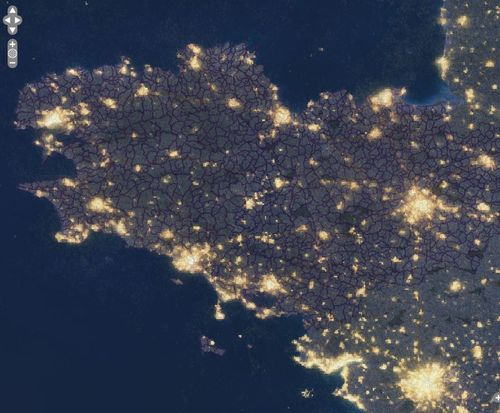
\includegraphics{bretagne.jpg}\hfill}

Voici ensuite les données générées grâce à cette image :

{\hfill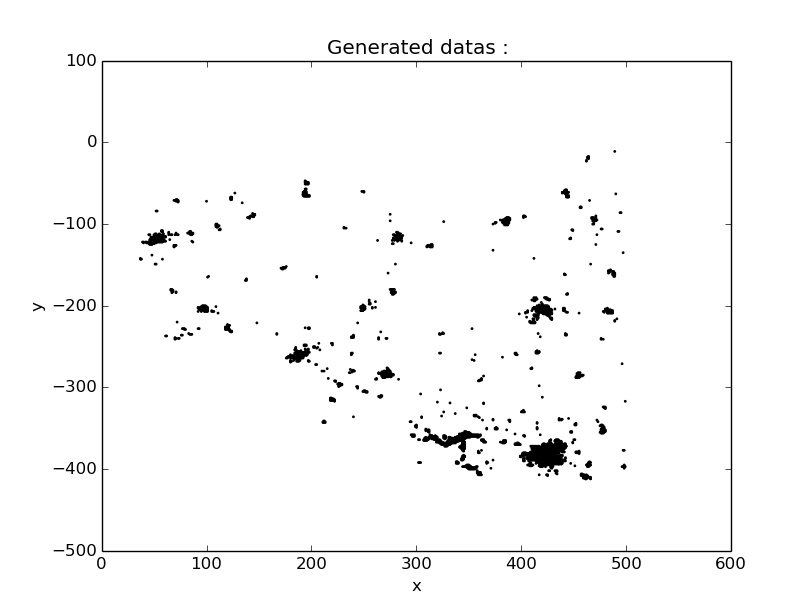
\includegraphics{bretagne_genData.png}\hfill}

Et enfin voici le résultat de kmeans sur ces images :

{\hfill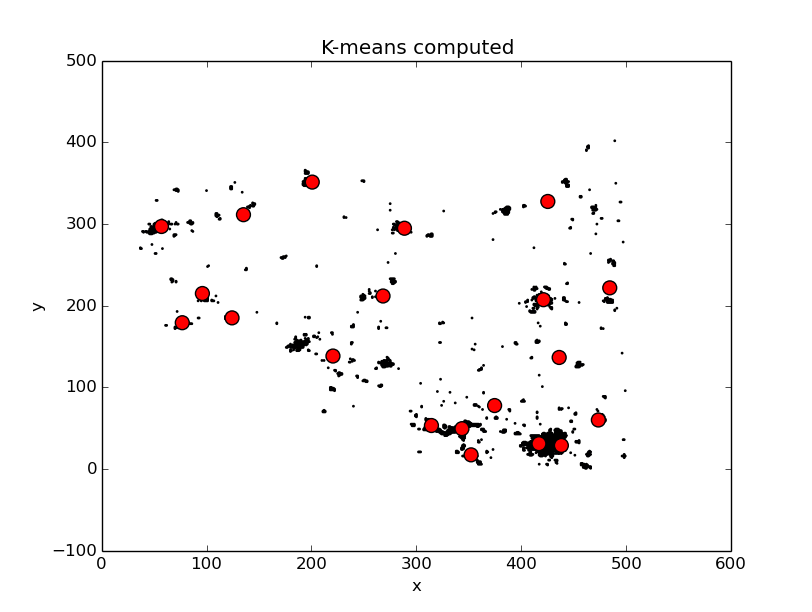
\includegraphics{bretagne_traitedData.png}\hfill}
\begin{itemize}
\item {} 
\DUspan{xref,std,std-ref}{genindex}

\item {} 
\DUspan{xref,std,std-ref}{modindex}

\item {} 
\DUspan{xref,std,std-ref}{search}

\end{itemize}


\renewcommand{\indexname}{Python Module Index}
\begin{theindex}
\def\bigletter#1{{\Large\sffamily#1}\nopagebreak\vspace{1mm}}
\bigletter{e}
\item {\texttt{es}}, \pageref{data:module-es}
\indexspace
\bigletter{k}
\item {\texttt{kmeans}}, \pageref{impl:module-kmeans}
\end{theindex}

\renewcommand{\indexname}{Index}
\printindex
\end{document}
